%%%%%%%%%%%%%%%%%%%%%%%%%%%%%%%%%%%%%%%%%
% a0poster Landscape Poster
% LaTeX Template
% Version 1.0 (22/06/13)
%
% The a0poster class was created by:
% Gerlinde Kettl and Matthias Weiser (tex@kettl.de)
% 
% This template has been downloaded from:
% http://www.LaTeXTemplates.com
%
% License:
% CC BY-NC-SA 3.0 (http://creativecommons.org/licenses/by-nc-sa/3.0/)
%
%%%%%%%%%%%%%%%%%%%%%%%%%%%%%%%%%%%%%%%%%

%----------------------------------------------------------------------------------------
%	PACKAGES AND OTHER DOCUMENT CONFIGURATIONS
%----------------------------------------------------------------------------------------

\documentclass[a0,landscape]{a0poster}

\usepackage{multicol} % This is so we can have multiple columns of text side-by-side
\columnsep=100pt % This is the amount of white space between the columns in the poster
\columnseprule=3pt % This is the thickness of the black line between the columns in the poster

\usepackage[svgnames]{xcolor} % Specify colors by their 'svgnames', for a full list of all colors available see here: http://www.latextemplates.com/svgnames-colors

\usepackage{times} % Use the times font
%\usepackage{palatino} % Uncomment to use the Palatino font

\usepackage{graphicx} % Required for including images
\graphicspath{{figures/}} % Location of the graphics files
\usepackage{booktabs} % Top and bottom rules for table
\usepackage[font=small,labelfont=bf]{caption} % Required for specifying captions to tables and figures
\usepackage{amsfonts, amsmath, amsthm, amssymb} % For math fonts, symbols and environments
\usepackage{wrapfig} % Allows wrapping text around tables and figures

\usepackage{natbib}

\begin{document}

%----------------------------------------------------------------------------------------
%	POSTER HEADER 
%----------------------------------------------------------------------------------------

% The header is divided into three boxes:
% The first is 55% wide and houses the title, subtitle, names and university/organization
% The second is 25% wide and houses contact information
% The third is 19% wide and houses a logo for your university/organization or a photo of you
% The widths of these boxes can be easily edited to accommodate your content as you see fit

\begin{minipage}[b]{0.75\linewidth}
\veryHuge \color{NavyBlue} \textbf{Pleiotropy vs. Close Linkage in the Diversity Outbred Mouse Study} \color{Black}\\ % Title
%\Huge\textit{An Exploration of Complexity}\\[1cm] % Subtitle
\huge \textbf{Fred Boehm, Mark Keller, Alan Attie, Gary Churchill, Brian Yandell, and Karl Broman}\\ % Author(s)
\huge University of Wisconsin-Madison \& The Jackson Laboratory\\ % University/organization
\end{minipage}
%
\begin{minipage}[b]{0.5\linewidth}
\color{DarkSlateGray}\Large \textbf{Contact Information:}\\
Department of Statistics\\ % Address
University of Wisconsin-Madison\\
%1220 Medical Sciences Center, 1300 University AVE\\
Email: \texttt{fred.boehm@wisc.edu}\\ % Email address
\end{minipage}
%
%\begin{minipage}[b]{0.19\linewidth}
%
\includegraphics[width=10cm]{logo.png} % Logo or a photo of you, adjust its dimensions here
%\end{minipage}

\vspace{1cm} % A bit of extra whitespace between the header and poster content

%----------------------------------------------------------------------------------------

\begin{multicols}{4} % This is how many columns your poster will be broken into, a poster with many figures may benefit from less columns whereas a text-heavy poster benefits from more

%----------------------------------------------------------------------------------------
%	ABSTRACT
%----------------------------------------------------------------------------------------

\color{Navy} % Navy color for the abstract

\begin{abstract}

We present initial results from our studies to differentiate pleiotropic QTl from closely linked QTL. In the context of univariate QTL mapping studies, we found numerous loci that associated with multiple clinical traits. To better understand the nature of these associations, we sought to distinguish pleiotropic effects, in which a single locus associates with multiple traits, from closely linked, but distinct, loci, in which two nearby genetic loci each associate with a single trait. We present a likelihood ratio test to quantitatively assess pleiotropy vs. close linkage for two traits that map to a small genomic region. 

\end{abstract}

%----------------------------------------------------------------------------------------
%	INTRODUCTION
%----------------------------------------------------------------------------------------

\color{SaddleBrown} % SaddleBrown color for the introduction
\section*{Introduction}

Methods for distinguishing a single pleiotropic genomic locus from multiple, closely linked loci have significant implications in modern genetics research. Such strategies may reveal novel roles for known genes and may contribute to discovery of previously unstudied genes. In both cases, our methods clarify the genetic underpinnings of complex traits. 


\begin{center}\vspace{1cm}
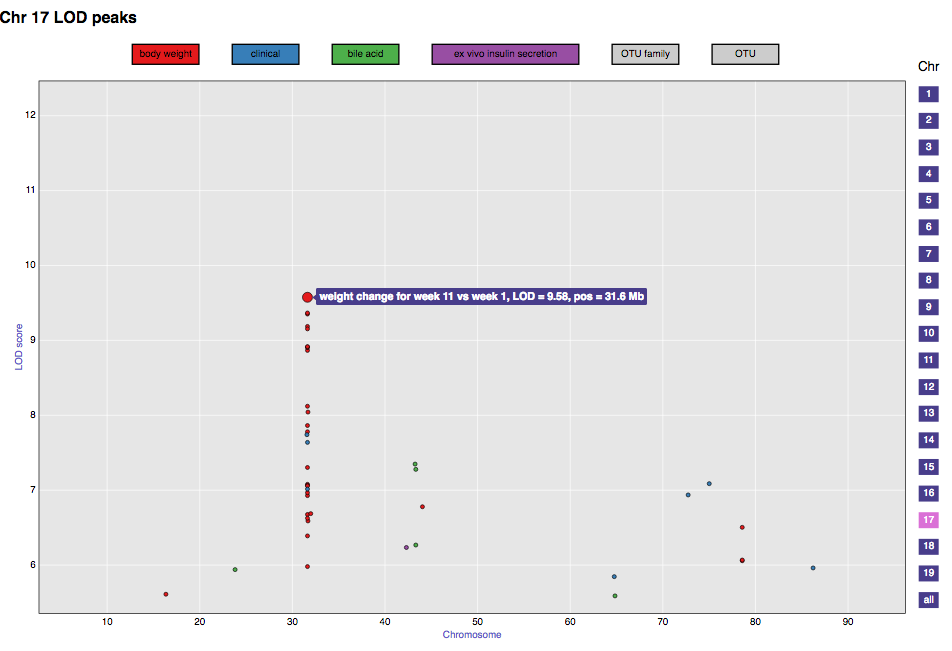
\includegraphics[width=0.8\linewidth]{lods-chr17}
\captionof{figure}{\color{Green} DO study LOD peaks on chromosome 17}
\end{center}\vspace{1cm}


%----------------------------------------------------------------------------------------
%	OBJECTIVES
%----------------------------------------------------------------------------------------

\color{DarkSlateGray} % DarkSlateGray color for the rest of the content

\section*{Approach}

\begin{enumerate}
\item Develop a likelihood ratio test (LRT) for the competing hypotheses, pleiotropy and close linkage
\item Implement the LRT in the R statistical computing environment 
\item Assess LRT performance with simulated data
\item Assess LRT performance with DO mouse phenotypes
\end{enumerate}

%----------------------------------------------------------------------------------------
%	MATERIALS AND METHODS
%----------------------------------------------------------------------------------------

\section*{Methods}

\subsection*{Likelihood ratio test development}

We first sought to implement a likelihood ratio test for the competing hypotheses:

\begin{eqnarray}
H_0: & \lambda_1 = \lambda_2\nonumber \\
H_a: & \lambda_1 \neq \lambda_2\nonumber
\end{eqnarray}

We initially limit our analysis to two traits of interest. This limitation simplifies calculations while still providing a platform from which to investigate more complicated scenarios. In the above hypotheses, $\lambda_1$ is the genomic location for the first QTL, while $\lambda_2$ is the QTL for the second QTL. By restricting the two loci to be the same, we have set the null hypothesis to be equivalent to pleiotropy. On the other hand, by allowing the two loci to differ, the alternative hypothesis represents close linkage.

We modeled the two phenotypes, together, as arising from normal distributions that depend on the estimated founder haplotype probabilities.

\begin{equation}
Y = XB + E
\end{equation}

where $Y$ is a n x 2 matrix of phenotype values, $X$ is the n x 8 matrix that includes a column of ones and 7 of the 8 estimated haplotype probabilities, $B$ is the 8 x 2 matrix of effect sizes, and $E$ is the n x 2 matrix of residuals.

Our LRT statistic then simplifies to the following:

\begin{equation}
\log \Lambda = - \frac{n}{2}\log \left( \frac{|\Sigma_0|}{|\Sigma_a|}\right)
\end{equation}

where $\Sigma_0$ and $\Sigma_a$ are the 2 x 2 matrices that's analogous to the sum of squared residuals in univariate regression, under, respectively, the null hypothesis and the alternative hypothesis.  


\subsection*{R implementation of LRT}

We implemented the calculations in the pleiotropy R package \cite{boehm2016}, which is available on github. 


%----------------------------------------------------------------------------------------
%	RESULTS 
%----------------------------------------------------------------------------------------

\section*{Results with simulated data}



\section*{Results with DO phenotypes}




\section*{Discussion}


%----------------------------------------------------------------------------------------
%	CONCLUSIONS
%----------------------------------------------------------------------------------------

\color{SaddleBrown} % SaddleBrown color for the conclusions to make them stand out

\section*{Conclusions}

\begin{itemize}
\item Pellentesque eget orci eros. Fusce ultricies, tellus et pellentesque fringilla, ante massa luctus libero, quis tristique purus urna nec nibh. Phasellus fermentum rutrum elementum. Nam quis justo lectus.
\item Vestibulum sem ante, hendrerit a gravida ac, blandit quis magna.
\item Donec sem metus, facilisis at condimentum eget, vehicula ut massa. Morbi consequat, diam sed convallis tincidunt, arcu nunc.
\item Nunc at convallis urna. isus ante. Pellentesque condimentum dui. Etiam sagittis purus non tellus tempor volutpat. Donec et dui non massa tristique adipiscing.
\end{itemize}

\color{DarkSlateGray} % Set the color back to DarkSlateGray for the rest of the content

%----------------------------------------------------------------------------------------
%	FORTHCOMING RESEARCH
%----------------------------------------------------------------------------------------

\section*{Forthcoming Research}



 %----------------------------------------------------------------------------------------
%	REFERENCES
%----------------------------------------------------------------------------------------


\bibliographystyle{plain} % Plain referencing style
\bibliography{sample} % Use the example bibliography file sample.bib

%----------------------------------------------------------------------------------------
%	ACKNOWLEDGEMENTS
%----------------------------------------------------------------------------------------

%\section*{Acknowledgements}

%Etiam fermentum, arcu ut gravida fringilla, dolor arcu laoreet justo, ut imperdiet urna arcu a arcu. Donec nec ante a dui tempus consectetur. Cras nisi turpis, dapibus sit amet mattis sed, laoreet.

%----------------------------------------------------------------------------------------

\end{multicols}
\end{document}